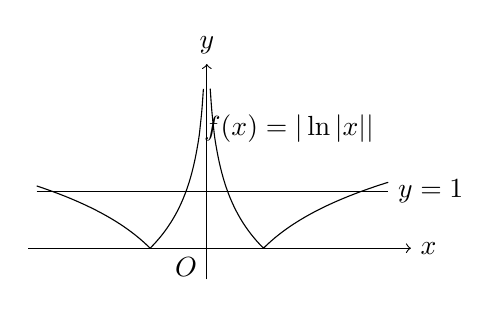
\begin{tikzpicture}[x=.72cm,y=.72cm,baseline=(current bounding box.center)]
  \draw[->] (-3.15,0)--(3.60,0) node[right] {$x$}; \draw[->] (0,-.55)--(0,3.25) node[above] {$y$};
  \draw[domain=-3.0:-.06,samples=120,smooth] plot (\x,{abs(ln(abs(\x)))});
  \draw[domain=.06:3.20,samples=120,smooth] plot (\x,{abs(ln(\x))});
  \draw (-3.0,1)--(3.20,1) node[right] {$y=1$};
  \node[below left] at (0,0) {$O$}; \node[above] at (1.45,1.70) {$f(x)=|\ln|x||$};
\end{tikzpicture}
